
\fancyhead[C]{Section 14.3}
\fancyhead[R]{\daynine}

\section*{\centering Chapter 14.3: Partial Derivatives}

\subsection*{Mechanics}
\begin{enumerate}
    \item \question{ %question
	Find all first and second partial derivatives for $f(x,y)=e^x+x\ln (y).$
	}
	{ %answer
	\[ f_x = e^x + \ln(y), \quad f_y = \frac{x}{y} \]
	\[ f_{xx} = e^x, \quad f_{xy} = \frac{1}{y} = f_{yx}, \quad f_{yy} = -\frac{x}{y^2} \]
	}
	{ %solution

	}

    \item \question{
		Find $f_x$, $f_y$, $f_z$, and $f_{xzz}$ for the function $f(x,y,z)=x\sin(yz)$.
	}
	{ %answer
	\[ f_x=\sin(yz),\quad f_y=xz\cos(yz),\quad f_z=xy\cos(yz),\quad f_{xzz}=-y^2\sin(yz) \]
	}
	{ %solution

	}

	\item \question{Find the total derivative $Df$ at the given point for each function below. Remember that $Df$ is the matrix of (partial) derivatives of the function and if $f$ is a function from $\R^n$ to $\R^m$ then $Df$ is a $m\times n$ matrix.
	\begin{enumerate}
		\item $f(x)=2x^3+7$ at $x=2$.
		\item $\mathbf{f}(t)=\langle 2\cos(t), 2 \sin(t), t\rangle$ at $t=\pi/2$.
		\item $f(x,y)=\sqrt{y-x}$ at $(x,y)=(1,2)$.
		\item $f(x,y,z)=e^{2y-x}+z^2+4$ at $(x,y,z)=(1,2,3)$.
		\item $\mathbf{f}(s,t) = \langle 2s+3t, t-s\rangle$ at $(s,t)=(1,1)$.  
	
		\textbf{Note:} The graph of this function is a surface (in this case all of $\R^2$) parameterized by two variables just like the graph of the function in (b) is a curve parameterized by one variable - we'll see these more later!  Another way of thinking about this is that this is a \textit{change of variables} for $\R^2$ between the system of coordinates $(s,t)$ and $(x,y)$.
	\end{enumerate}
	}
	{ %answer
	\begin{multicols}{2}
		\begin{enumerate}
		\item $Df(2)=f'(2)=[24]$
		\item $D\mathbf{f}(\pi/2)=\mathbf{f}'(\pi/2)=\begin{bmatrix}
			-2 \\ 0 \\ 1
		\end{bmatrix}$
		\item $Df(1,2)=\begin{bmatrix}
			-1/2 & 1/2
		\end{bmatrix}$
		\item $Df(1,2,3)=\begin{bmatrix}
			-e^3 & 2e^3 & 6
		\end{bmatrix}$
		\item $D\mathbf{f}(1,1) = \begin{bmatrix}
			2 & 3 \\
			-1 &  1
		\end{bmatrix}  $
	\end{enumerate}
	\end{multicols}
	}
	{ %solution

	}
    
\end{enumerate}
\subsection*{Applications}
\begin{enumerate}[resume]
    \item \question{
		The speed of sound $C$ traveling through ocean water is a function of 
	temperature, salinity, and depth.  It may be modeled by the function	
	\[C(T,S,D)=1450 +4.5T-0.05T^2+0.0003T^3+(1.5-0.01T)(S-35)+0.015D, \]
	
	where $C$ is the speed of sound in meters/second, $T$ is the temprature in degrees Celsius, $S$ is the salinity in grams/liter of water, and $D$ is the depth below the ocean surface in meters.
	
	\begin{enumerate}
		\item State the units in which each of the partial derivatives $C_T,C_S,$ and $C_D$ are expressed and explain the physical meaning of each.
		
		\item Find the partial derivatives $C_T, C_S,$ and $C_D$.
		
		\item Evaluate each of the three partial derivatives at the point where $T=10, S=35$, and $D=100$.  What does the sign of each partial derivative tell us about the behavior of the function $C$ at the point $(10,35,100)$?
	\end{enumerate}
	}
	{ %answer
	\begin{enumerate}
		\item $C_T$: (meters/second)/ degree Celsius - this gives the change in speed for each one degree C of temperature increase.
		$C_S$ (meters/second)/(grams/liter) - this gives the change in speed for each one gram/liter increase in salinity
		$C_D$: (meters/second)/meter - this gives the change in speed for each one meter increase in depth below the surface
		
		\item $C_T= 4.5-0.1T+0.0009T^2-0.01(S-35)$
		$C_S=1.5-0.01T$
		$C_D=0.015$
		
		\item At $(T,S,D)=(10,35,100)$, we have $C_T=3.59, C_S=1.4, C_D=0.015$.  This tells us that if we increase the temperature, salinity, or depth from these conditions the speed of sound will increase as well.
	\end{enumerate}
	}
	{ %solution
	} 
    
    \item \question{Recall from last week's worksheet that a utility function is a multivariable function $u(x,y,z)$, where $x,y,z$ represent three independent properties of an object (eg., price, quantity, quality), and $u$ tells you how much you value that item. The \textit{marginal utility functions} are the partial derivatives $u_x,u_y$ and $u_z$. What is the economic interpretation of the marginal utilities?}
    { %answer
	The marginal utility functions tell you how much your utility (value) changes when you change one of the properties of the object, while keeping the other two properties fixed.
	}
	{ %solution
	}
\end{enumerate}
\subsection*{Extensions}
\begin{enumerate}[resume]
	
	\item \question{
		Below is a contour plot for a function $f(x,y)$, with values for some of the contours (level curves) indicated on the \textit{left} of the figure.
	
	\begin{minipage}{0.6\textwidth}
		\begin{enumerate}
			\item Find the sign of the partial derivatives \\
            $f_x(-2,-1)$ and $f_y(-2,-1)$.
			\item At the point $(0,-1/2)$, which is larger? $f_x$ or $f_y$?
			\item Find all $(x,y)$ where $f_x(x,y)=0$.
			\item Locate, if possible, one point $(x,y)$ where\\ $f_x(x,y)<0$.
		\end{enumerate}
	\end{minipage}
	\begin{minipage}{0.4\textwidth}
		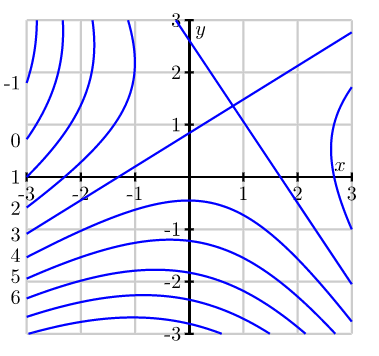
\includegraphics[scale=0.6, alt={A contour plot on a grid with x and y from -3 to 3. The plot displays multiple level curves. In the lower half, a series of downward-opening hyperbolas are labeled with values increasing from 1 to 6. In the upper half, the curves resemble hyperbolas opening to the left. Near (1,1)), the contours form a saddle point, highlighted by two intersecting straight lines surrounded by hyperbolic curves.}]{contour_14_3.png}
	\end{minipage}
	}{ %answer
	\begin{enumerate}
		\item $f_x(-2,-1)>0$ and $f_y(-2,-1)<0$
		\item $f_y(0,-1/2)>f_x(0,-1/2)$
		\item $f_x(x,y)=0$ along the tops of the arcs labeled $4,5,6,...$
		\item One such point is $(1,-3/2)$
	\end{enumerate}
	}
	{ %solution
	}

	\item \question{The fifth-order partial derivative $\partial^5f/\partial x^2\partial y^3$ is zero for each of the following functions.  To show this as quickly as possible, which variable would you differentiate with respect to first: $x$ or $y$?
	
	Try to answer without writing anything down.  Why did you make the choice you did?
	
	\begin{enumerate}
		\item $f(x,y)=y^2x^4e^x+2$
		
		\item $f(x,y)=y^2+y(\sin(x)-x^4)$
		
		\item $f(x,y)=x^2+5xy+\sin(x)+7e^x$
		
		\item $f(x,y)=xe^{y^/2}$
	\end{enumerate}}
	{ %answer
		Note this does not have a definitive right answer - some differences may arise and that's good! Discuss!
	
	\begin{enumerate}
		\item First $y$ since $\partial^3 f/\partial y^3=0$ and the $y$-partial derivatives are easier
		
		\item First $y$, since $\partial^3 f/\partial y^3=0$
		
		\item First $y$, since $\partial^2 f/\partial y^2=0$
		
		\item First $x$, since $\partial^2 f/\partial x^2=0$ and the $x$-partial derivatives are easier.
	\end{enumerate}
	
	A common theme is to work with the variable with lower powers/simpler expressions first when taking mixed partials.
	}
	{ %solution
	}

    \item Let $A$ be any $2\times 2$ matrix, and let $\mathbf{f}: \mathbb{R}^2\to\mathbb{R}^2$ be given by $\mathbf{f}(\mathbf{x}) = A\mathbf{x}$. Compute the total derivative $D\mathbf{f}$. What do you notice? What familiar family of functions from Calc 1 does this remind you of? Can you generalize this result? 
\end{enumerate}